\documentclass[
		11pt,
		a4paper,
		toc=listof, %% Abbildungs-, Tabellenverzeichnis mit ins Inhaltsverzeichni
		bibliography=totoc %% Quellenverzeichnis mit ins Inhaltsverzeichnis
		]{scrreprt}	 %% KOMA Script

% HTWG
\usepackage{graphicx}
\usepackage{a4}
\usepackage{german}

% Eigene
\usepackage[utf8]{inputenc} %% Umlaute
\usepackage[printonlyused]{acronym} %% Abkuerzungsverzeichnis (nur verwendete)
\usepackage{todonotes} %% TODOs moeglich mit \todo{}
\usepackage{booktabs} %% Tabellen
\usepackage{amsmath} %% Formeln
\usepackage{listings} %% Codebeispiele
\usepackage{subfigure} %% Mehrere Bilder nebeneinander
\usepackage{hyperref} %% referenzen innerhalb und außerhalb des Dokumentes

% Eigenes Design
%TODO loeschen wenn default HTWG Design (was es nicht wirklich gibt) gewuuenscht ist
\usepackage[bottom=3cm]{geometry}
\usepackage{setspace}
\onehalfspacing


% KOMA script anpassungen
%TODO entfernen wenn kein KOMA Script gewuenscht
\usepackage{scrhack}

%%%%%%%% Codebeispiele
\usepackage{color}
\usepackage{xcolor}
\usepackage{listings}
\usepackage{caption}

\setcounter{tocdepth}{2}  %% Uebreschriften bis subsectionw ins Inhaltsverzeichnis
\setcounter{secnumdepth}{2}  %% Nummerierung bis subsection


%%% Codebeispiele - Style
\lstdefinestyle{mystyle}{
    basicstyle=\footnotesize,
    aboveskip=10pt,
    breakatwhitespace=false,
    breaklines=true,
    captionpos=b,
    belowcaptionskip=5pt,
    keepspaces=true,
    numbers=left,
    numbersep=15pt,
    showspaces=false,
    showstringspaces=false,
    showtabs=false,
    tabsize=2,
    frame=single,
    lineskip=-0.4pt,
    framexleftmargin=0.5em,
    xleftmargin=2.5em
}
\lstset{style=mystyle}


% Entfernt Kapitel Ueberschrift
% Bsp.
% 	ALT:
%       Kapitel 1
%       Einführung
%
% 	NEU:
% 		1 Einführung
%
\renewcommand*\chapterheadstartvskip{\vspace{-\topskip}}


% Hurenkind und Schusterjunge vermeiden
\clubpenalty = 10000 % schliesst Schusterjungen aus
\widowpenalty = 10000 \displaywidowpenalty = 10000% schliesst Hurenkinder aus


% Alle Listen mit einem "-" statt einem Punkt
\def\labelitemi{--}


\newcommand{\thema}{$[$Thema der Bachelorarbeit$]$}
\newcommand{\schlagworte}{$[$Platz, f\"ur, spezifische, Schlagworte, zur, Ausarbeitung $]$}
\newcommand{\zusammenfassung}{$[$Text der Zusammenfassung etwa 150 Worte. Es soll der
	L"osungsweg beschrieben sein.$]$}
\newcommand{\ausgabedatum}{$[$Datum$]$}
\newcommand{\abgabedatum}{15.02.2016}
\newcommand{\autor}{Sandro Tonon}
\newcommand{\autorStrasse}{Allemannenstra"se 10}
\newcommand{\autorPLZ}{78467}
\newcommand{\autorOrt}{Konstanz}
\newcommand{\autorGeburtsort}{Waldshut-Tiengen}
\newcommand{\autorGeburtsdatum}{02.07.1990}
\newcommand{\prueferA}{Prof. Dr. Marko Boger}
\newcommand{\prueferB}{Dipl. Ing. Andreas Maurer}
\newcommand{\firma}{Seitenbau GmbH}
\newcommand{\studiengang}{Angewandte Informatik}



\begin{document}
%% Nummerierung aus
\pagenumbering{gobble}

% HTWG Tempaltes fuer Titelseite etc.

\begin{titlepage}

\vspace*{-3.5cm}

\begin{flushleft}
\hspace*{-1cm} 
\includegraphics[width=15.7cm]{htwg-logo}
\end{flushleft}

\vspace{2.5cm}

\begin{center}
	\huge{
		\textbf{\thema} \\[5cm]
	}
	\Large{
		\textbf{\autor}} \\[6.5cm]
	\large{
		\textbf{Konstanz, \abgabedatum} \\[2.3cm]
	}
	
	\Huge{
		\textbf{{\sf BACHELORARBEIT}}
	}
\end{center}

\end{titlepage}

\thispagestyle{empty}
{
\setlength{\parskip}{0.5cm}
        \begin{center}
        \textbf{\huge BACHELORARBEIT}

        \textbf{zur Erlangung des akademischen Grades}

        \textbf{\Large Bachelor of Science (B. Sc.)}

        \textbf{an der}

        \textsf{\huge Hochschule Konstanz}\\
        {\small Technik, Wirtschaft und Gestaltung}

        \textsf{\Large Fakult"at Informatik} \\
        Studiengang \studiengang
        \end{center}
}
\begin{center}

\vspace*{2cm}

\begin{tabular}{p{3cm}p{10cm}}
Thema: & \multicolumn{1}{l}{\textbf{\large \thema}} \\[15ex]
Bachelorkandidat: & \autor, \autorStrasse, \autorPLZ{}  \autorOrt{} \\[15ex]
1. Pr"ufer: & \prueferA \\
2. Pr"ufer: & \prueferB \\[25ex]
Ausgabedatum: & \ausgabedatum \\
Abgabedatum: & \abgabedatum \\
\end{tabular}
\end{center}

\begin{center}
{\Large \textbf{Zusammenfassung (Abstract)}}
\end{center}

\bigskip

\begin{center}
	\begin{tabular}{p{2.8cm}p{10cm}}
		Thema: & \thema \\
		 & \\
		Bachelorkandidat: & \autor \\
		 & \\
		Firma: & \firma \\
		 & \\
		Betreuer: & \prueferA  \\[.5ex]
		 &  \prueferB \\
		 & \\
		Abgabedatum: & \abgabedatum \\
		 & \\
		Schlagworte: & \schlagworte \\
		 & \\
	\end{tabular}
\end{center}

\bigskip

\noindent
\zusammenfassung

\pagenumbering{Roman}
\chapter*{Ehrenw"ortliche Erkl"arung}
\addcontentsline{toc}{chapter}{Ehrenw"ortliche Erkl"arung}

Hiermit erkl"are ich
\textit{\autor, geboren am \autorGeburtsdatum{} in \autorGeburtsort{}}, dass ich\\

\begin{tabular}{lp{12cm}}
(1) & meine Bachelorarbeit mit dem Titel \\[1em]
& \textbf{\thema} \\[1em]
& selbstst"andig und ohne fremde Hilfe angefertigt und keine anderen als die angef"uhrten Hilfen benutzt habe;\\[1em]
(2) & die "Ubernahme w"ortlicher Zitate, von Tabellen, Zeichnungen, Bildern und
Programmen aus der Literatur oder anderen Quellen (Internet) sowie die Verwendung
der Gedanken anderer Autoren an den entsprechenden Stellen innerhalb der Arbeit
gekennzeichnet habe.\\
\end{tabular}

\vspace*{1cm}

\noindent
Ich bin mir bewusst, dass eine falsche Erkl"arung rechtliche Folgen haben wird.\\

\vspace*{3cm}

\noindent
Konstanz, \abgabedatum \hfill \begin{tabular}{c} \\ \\ \rule{5cm}{1pt} \\ (Unterschrift)\end{tabular}


\tableofcontents

% Literaturverzeichnis
\section{Abkürzungsverzeichnis}
\begin{acronym}

 \acro{bzw.}{beziehungsweise}
 \acro{HTML}{Hypertext Markup Language}
 \acro{W3C}{World Wide Web Consortium}
 \acro{DOM}{Document Object Model}
 \acro{CSS}{Cascading Style Sheets}
 \acro{API}{Application Programming Interface}
 \acro{FOUC}{Flash Of Unstyled Content}
 \acro{LIFO}{Last In First Out}

\end{acronym}
\end{document}


%% Starte Paginierung
\cleardoublepage
\pagenumbering{arabic}

\chapter{Einleitung}\label{einleitung}

Der Begriff ``Web Components'' ist ein Dachbegriff für mehrere entstehende Standards \cite{citeulike:13844988}, welche es für Webentwickler ermöglichen sollen, komplexe Anwendungsentwicklungen mit einer neuen Sammlung an Werkzeugen zu vereinfachen. Diese sollen die Wartbarkeit, Interoperabilität und Kapselung verbessern und somit ein Plugin-System für das Web schaffen. Durch die neuen Standards soll das Web zu einer Plattform werden, die es ermöglicht, die Web-Sprache \ac{HTML} zu erweitern. Dies ist bisher nicht möglich, da die \ac{HTML}-Technologie - und somit die Möglichkeiten, \ac{HTML}-Tags zu benutzen - vom \ac{W3C} definiert und standardisiert wird. Unter den wichtigsten der neuen Standards sind die folgenden 4 Technologien aufzuführen: Custom Elements, Shadow \ac{DOM}, \ac{HTML} Templates und \ac{HTML} Imports. Custom Elements ermöglichen es einem Webentwickler, eigene \ac{HTML}-Tags und deren Verhalten zu definieren, oder bereits vorhandene oder native \ac{HTML}-Tags zu erweitern. Das Shadow \ac{DOM} stellt ein Sub-\ac{DOM} in einem \ac{HTML}-Element bereit, welches dem Element zugehöriges Markup, \ac{CSS} und JavaScript kapselt. \ac{HTML} Templates stellen, wie der Name impliziert, einen Template-Mechanismus für \ac{HTML} bereit und \ac{HTML} Imports erlauben das Laden von \ac{HTML}-Dokumenten in andere \ac{HTML}-Dokumente. \cite{citeulike:13842702}, \cite{citeulike:13842701}

Diese neuen Technologien werden allerdings noch nicht vollständig von allen populären Browsern, zu welchen Google Chrome, Mozilla Firefox, Opera und der Internet Explorer bzw. Edge, gehören, unterstützt. Des Weiteren ist das Implementieren einer Applikation, welche diese Technologien nativ benutzt, bisher sehr komplex und schwierig zu organisieren. Im Zuge dessen, entwickelt Google aktiv an einer Library namens Polymer, welche sich diesen Problemen annimmt.
Polymer stellt dabei eine Reihe an unterschiedlichen Schichten dar, welche den Umgang mit Web Components vereinfachen sollen. So stellt Polymer eine Sammlung an Mechanismen bereit, welche älteren Browsern die nötigen Features für den Einsatz von Web Components beibringen. Ebenso soll das Erstellen von eigenen \ac{HTML}-Elementen mit der Polymer-Library und der damit bereitgestellten \ac{API} für Entwickler komfortabler gemacht werden. Um bereits entwickelte Web Components einfach wiederverwenden zu können, bietet Polymer eine Sammlung von vorgefertigten Elementen an.

Web Components und die Polymer-Library greifen stark in den Entwicklungsprozess von Webseiten ein und sollen diesen verbessern und vereinfachen. Die Seitenbau GmbH interessiert sich stark für diese neue Technologie, da Wiederverwendbarkeit, Wartbarkeit und neue Technologien im Fokus des Frontend-Engineerings des Unternehmens stehen.
Die Seitenbau GmbH ist ein mittelständischer IT-Dienstleister und unterstützt seit 1996 Organisationen aus Privatwirtschaft und öffentlicher Verwaltung bei der Planung, Konzeption und Umsetzung hochwertiger Softwarelösungen für E-Business und E-Government. Zu den Kernkompetenzen der Seitenbau GmbH zählen dabei vor allem das Frontend Engineering und Content Management, die Konzeption und Entwicklung von Individualsoftware sowie der Aufbau von personalisierten Intranet- und Portallösungen.

Im Rahmen dieser Bachelorarbeit sollen die verschiedenen Technologien unter dem Dachbegriff Web Components sowie deren Funktionsweise sowohl ohne, als auch mit der Polymer-Library, untersucht werden. Zur Veranschaulichung soll eine Web Component mit Hilfe von Polymer implementiert und mit einer ähnlichen Implementierung mit AngularJS verglichen werden. Am Beispiel einer Web Component in Form einer Multi-Navigations-Applikation sollen die Vor- und Nachteile des Einsatzes von Polymer in Hinblick auf Implementierung und Performance dargestellt werden.

In Kapitel \ref{web-components-nach-w3c} werden die Standards der Web Components beschrieben, auf welche die in Kapitel \ref{einfuehrung-in-polymer} beschriebene Library Polymer aufsetzt. Wie sie dies im Detail umsetzt wird in Kapitel \ref{analogie-zu-nativen-web-components} beschrieben. In Kapitel \ref{zusaetzliche-polymer-funktionalitaeten} werden zusätzliche Funktionalitäten dieser Library aufgezeigt und in Kapitel \ref{best-practices-beim-arbeiten-mit-polymer} werden einige Best Practices im Umgang mit ihr erklärt. Die in den Kapiteln \ref{einfuehrung-in-polymer} bis \ref{best-practices-beim-arbeiten-mit-polymer} gewonnenen Erkenntnisse werden in Kapitel \ref{komponenten-entwicklung} in einer Beispielimplementierung umgesetzt und mit einer ähnlichen Implementierung mit AngularJS verglichen. In Kapitel \ref{zukunftsprognose} wird abschließend eine Zukunftsprognose aufgestellt.


\section{Polyfills}\label{polyfills-mit-webcomponents.js}

In den Abschnitten \ref{custom-elements} bis \ref{html-imports} wurde gezeigt, wie die Web-Components-Technologien funktionieren und ob diese bereits in allen Browsern unterstützt werden. In diesem Abschnitt wird genauer darauf eingegangen was Polyfills sind. Ebenso wird auf deren Performance eingegangen und wie sie die Browserunterstützung der Web-Components-Technologien verbessern.


\subsection{Native Browserunterstützung von Web Components}\label{native-browserunterstuxfctzung-von-web-components}

In den einzelnen Unterkapiteln zu den Technologien wurde jeweils kurz gezeigt, ob diese von den Browsern unterstützt wird oder nicht. Es wurde deutlich, dass Chrome und Opera bisher die einzigen Vorreiter sind. Bis auf \ac{HTML} Templates, welche von allen modernen Browsern unterstützt werden, unterstützen sie als einzige alle Technologien. \cite{citeulike:13914379}

\begin{description}
  \item[Chrome] Hat alle Spezifikationen der Web-Component-Standards ab Version 43 komplett implementiert.
  \item[Firefox] Unterstützt nativ \ac{HTML} Templates. Custom Elements und Shadow \ac{DOM} sind zwar implementiert, müssen aber über das Flag \texttt{dom.webcomponents.enabled} manuell in den Entwicklereinstellungen aktiviert werden. \ac{HTML} Imports werden, wie in Kapitel \ref{html-imports} erwähnt, bis auf Weiteres nicht unterstützt.
  \item[Safari] \ac{HTML} Templates werden ab Version 8 unterstützt, Custom Elements und Shadow \ac{DOM} befinden sich in der Entwicklung (Stand Januar 2016), \ac{HTML} Imports werden jedoch nicht unterstützt.
  \item[Internet Explorer] Als einziger Browser unterstützt der Internet Explorer keine der Web-Components-Technologien. Die Unterstützung wird -- auf Grund der Einstellung der Entwicklung und des Wechsels zu Microsoft Edge -- auch nicht nachträglich implementiert werden.
  \item[Microsoft Edge] Templates werden ab Version 13 unterstützt, über die Entwicklung der restlichen Technologien kann allerdings abgestimmt werden \cite{citeulike:13914237}.
  \item[Mobile Browser] Alle Technologien werden bisher nur auf Android in den Browsern Chrome für Android, Opera und Android Browser unterstützt.
\end{description}

Die Browserunterstützung der Technologien der Web Components ist momentan also noch verhalten. Das bedeutet jedoch nicht, dass sie noch nicht verwendet werden können. Mittels JavaScript besteht die Möglichkeit, die Technologien den Browsern beizubringen, welche sie nicht unterstützen. Ein solches JavaScript wird ``Polyfill'' genannt.


\subsection{Polyfill webcomponents.js}\label{polyfill-webcomponents.js}

\begin{quote}
A polyfill, or polyfiller, is a piece of code (or plugin) that provides the technology that you, the developer, expect the browser to provide natively. \cite{citeulike:13914241}
\end{quote}

Mit Hilfe von Polyfills können die Technologie-Lücken der Browser also auf mehrere, unterschiedliche Arten (``Poly'') gefüllt (``fill'') werden \cite{citeulike:13914234}. Eine Sammlung an Polyfills Technologien der Web Components bildet das JavaScript webcomponents.js. Es wurde von Google im Rahmen von Polymer entwickelt und hat eine dermaßen weite Verbreitung erfahren, dass es auszugliedern wurde. Somit kann es auch unabhängig von der Benutzung von Polymer eingesetzt werden \cite{citeulike:13914239}.


\subsection{Browserunterstützung}\label{polyfills-browserunterstuetzung}

Mit dem Einsatz der webcomponents.js Polyfills werden die Web Components auch auf den Internet Explorer, Firefox sowie Safari portiert. Eine detaillierte Matrix der Browserunterstützung der Web Components mit Einsatz der Polyfills ist in Abbildung \ref{fig:bdwctmwcjs} \cite{citeulike:13914238} dargestellt.

\begin{figure}[htbp]
 \centering
 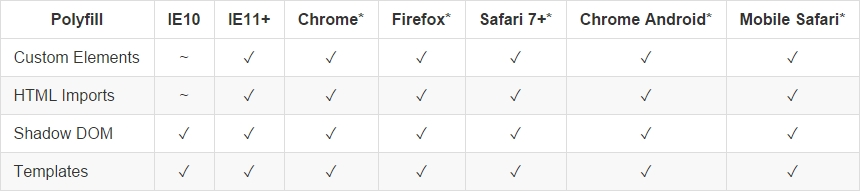
\includegraphics[width=\linewidth]{kapitel2/bilder/6-webcomponentsjs-browserunterstuetzung}
 \caption{Browserunterstützung der Web Components Technologien mit webcomponents.js}
 \label{fig:bdwctmwcjs}
\end{figure}

Jedoch werden die Technologien der Web Components auch mit Einsatzes der Polyfills nur von den aktuelleren Versionen des jeweiligen Browsers unterstützt. Darunter fallen jedoch weiterhin nicht ältere Browser, wie beispielsweise der Internet Explorer in Version 8 und 9. Des Weiteren werden einige Technologien auf Grund der Komplexität nicht komplett simuliert. Hier muss bei einigen Technologien auf folgende Punkte geachtet werden.

\begin{description}
  \item[Custom Elements] Die \ac{CSS}-Pseudoklasse \texttt{:unresolved} wird nicht unterstützt.
  \item[Shadow \ac{DOM}] Das Shadow \ac{DOM} kann auf Grund der Kapselung nicht komplett künstlich simuliert werden, dennoch versucht das webcomponents.js Polyfill einige der Features zu simulieren. So sprechen definierte \ac{CSS}-Regeln alle Elemente in einem künstlichen Shadow Root an -- als würde man den \texttt{\textgreater{}\textgreater{}\textgreater{}} Selektor benutzen -- auch die \texttt{::shadow} und \texttt{::content} Pseudoelemente verhalten sich so.
  \item[\ac{HTML} Templates] Templates, welche mit einem Polyfill erzeugt werden, sind nicht unsichtbar für den Browser, ihre enthaltenen Ressourcen werden also schon beim initialen Laden der Seite heruntergeladen.
  \item[\ac{HTML} Imports] Die zu importierenden \ac{HTML}-Dateien werden mit einem \ac{XHR}, und somit asynchron heruntergeladen, selbst wenn das \texttt{async}-Attribut (siehe Abschnitt \ref{asynchrones-laden-von-imports}) nicht gesetzt ist.
\end{description}


\subsection{Performance}\label{performance}

Das webcomponents.js-JavaScript \cite{citeulike:13914238} bringt mit seiner Größe von 116 KB einen großen Umfang mit, was sich negativ auf die Ladezeiten der Webseite auswirkt. Des Weiteren müssen die von den Browsern nicht unterstützten und ignorierten \ac{CSS}-Regeln -- wie \texttt{::shadow} oder \texttt{::slotted} -- mit Regular Expressions nachgebaut werden, was momentan 40 Stück sind. Das macht die Polyfills extrem komplex und träge. Die Funktionen zum Traversieren des \ac{DOM}s müssen angepasst werden, damit nur die richtigen Elemente angezeigt werden und eine Shadow Boundary simuliert wird. Diese werden mit 42 Wrappern umgesetzt, was wie die Regular Expressions zur Simulation der \ac{CSS}-Regeln sehr aufwändig ist. Allerdings können einige Funktionen wie \texttt{window.document} schlichtweg nicht überschrieben werden. Im Allgemeinen wird die \ac{DOM}-\ac{API} stark verlangsamt, wodurch die Performance -- speziell auf mobilen Geräten -- drastisch sinkt und mitunter nicht tolerierbar ist \cite{citeulike:13886251}.


\subsection{\texorpdfstring{Request-Minimierung mit ``Vulcanize''}{Request-Minimierung mit Vulcanize}}\label{request-minimierung-mit-vulcanize}

Webseiten können viele verschiedene, modular aufgebaute JavaScript-Dateien, Stylesheets, etc. beinhalten, welche die Anzahl an Requests erhöhen. Um die Anzahl an Requests zu verringern gibt es in der Webentwicklung bereits mehrere verschiedene Hilfsmittel. So werden die einzelnen Stylesheets oder auch JavaScript Dateien zu einer einzigen Datei konkateniert, sodass für das komplette Styling und JavaScript jeweils eine große Datei entsteht, welche nur einen Request an den Server benötigen. Zusätzlich kann sie anschließend noch minifiziert werden, um ihre Größe zu verringern und die Ladezeiten zu verkürzen. Selbiges Prinzip kann auch auf die \ac{HTML} Imports angewendet werden. Google stellt hierfür das Tool Vulcanize \cite{citeulike:13879681} bereit, welches serverseitig ermöglicht, einzelne kleine Web Components in einer einzigen, großen Web Component zusammenzufassen. Benannt nach der Vulkanisation, werden metaphorisch die einzelnen Elemente in ein beständigere Materialien umgewandelt. Vulcanize reduziert dabei eine \ac{HTML}-Datei und ihre zu importierenden \ac{HTML}-Dateien in eine einzige Datei. Somit werden die unterschiedlichen Requests in nur einem einzigen gebündelt und die Ladezeiten sowie die benötigte Bandbreite minimiert.



%!TEX root = ../thesis.tex

\chapter{Grundlagen}

\ac{LOL} Lorem ipsum dolor sit amet, consetetur sadipscing elitr, sed diam nonumy eirmod tempor invidunt ut labore et dolore magna aliquyam erat, sed diam voluptua. At vero eos et accusam et justo duo dolores et ea rebum. Stet clita kasd gubergren, no sea takimata sanctus est Lorem \ac{HTTP} ipsum dolor sit amet. Lorem ipsum dolor sit amet, consetetur sadipscing elitr, sed diam nonumy eirmod tempor invidunt ut labore et dolore magna aliquyam erat, sed diam voluptua. At vero eos et accusam et justo duo dolores et ea rebum. Stet clita kasd gubergren, no sea takimata sanctus est Lorem ipsum dolor sit amet.

\section{tbd} 

Lorem ipsum dolor sit amet, consetetur sadipscing elitr, sed diam nonumy eirmod tempor invidunt ut labore et dolore magna aliquyam erat, sed diam voluptua. At vero eos et accusam et justo duo dolores et ea rebum. Stet clita kasd gubergren, no sea takimata sanctus est Lorem ipsum dolor sit amet. Lorem ipsum dolor sit amet, consetetur sadipscing elitr, sed diam nonumy eirmod tempor invidunt ut labore et dolore magna aliquyam erat, sed diam voluptua. At vero eos et accusam et justo duo dolores et ea rebum. Stet clita kasd gubergren, no sea takimata sanctus est Lorem ipsum dolor sit amet.

\subsection{tbd} 
Lorem ipsum dolor sit amet, consetetur sadipscing elitr, sed diam nonumy eirmod tempor invidunt ut labore et dolore magna aliquyam erat, sed diam voluptua. At vero eos et accusam et justo duo dolores et ea rebum. Stet clita kasd gubergren, no sea takimata sanctus est Lorem ipsum dolor sit amet. Lorem ipsum dolor sit amet, consetetur sadipscing elitr, sed diam nonumy eirmod tempor invidunt ut labore et dolore magna aliquyam erat, sed diam voluptua. At vero eos et accusam et justo duo dolores et ea rebum. Stet clita kasd gubergren, no sea takimata sanctus est Lorem ipsum dolor sit amet.

\subsubsection{tbd} 
Lorem ipsum dolor sit amet, consetetur sadipscing elitr, sed diam nonumy eirmod tempor invidunt ut labore et dolore magna aliquyam erat, sed diam voluptua. At vero eos et accusam et justo duo dolores et ea rebum. Stet clita kasd gubergren, no sea takimata sanctus est Lorem ipsum dolor sit amet. Lorem ipsum dolor sit amet, consetetur sadipscing elitr, sed diam nonumy eirmod tempor invidunt ut labore et dolore magna aliquyam erat, sed diam voluptua. At vero eos et accusam et justo duo dolores et ea rebum. Stet clita kasd gubergren, no sea takimata sanctus est Lorem ipsum dolor sit amet.


\chapter{Web Components nach dem vorläufigen W3C-Standard}\label{web-components-nach-w3c}

In diesem Kapitel wird in Abschnitt \ref{problemloesung} auf die Problemlösung der Web Components nach den Vorstellungen des \ac{W3C} eingegangen. In Abschnitt \ref{custom-elements} wird die erste Technologie vorgestellt, die Custom Elements, Abschnitt \ref{html-templates} wird sich den \ac{HTML} Templates widmen, in Abschnitt \ref{shadow-dom} wird auf den Shadow \ac{DOM} eingegangen und in Abschnitt \ref{html-imports} wird die letzte Technologie, die \ac{HTML} Imports, gezeigt. In Abschnitt \ref{polyfills-mit-webcomponents.js} werden die, für diese Technologien entwickelten Polyfills erklärt. Abschließend wird in Kapitel \ref{implementierung-einer-komponente-mit-den-nativen-web-component-apis} eine exemplarische Komponente implementiert.


\section{Problemlösung}\label{problemloesung}

In der heutigen Webentwicklung kommt es häufig vor, dass für diverse Probleme oftmals die gleiche, oder eine ähnliche Lösung entwickelt werden muss. Diese unterscheiden sich stets leicht, bringen im Kern aber dennoch meist die selben Features mit sich. Um diese Features auf der Webseite verfügbar zu machen, sind eine Reihe an verschiedenen Technologien notwendig. Zum einen muss das von ihr benötigte \ac{HTML}-Markup geschrieben werden, zum anderen muss ein JavaScript eingebunden und über eine vorgegebene \ac{API} konfiguriert werden, damit das Feature überhaupt funktioniert. Damit die Komponente dann in das Design der eigenen Webseite einfügt, muss ebenso ein entsprechendes Stylesheet mit den Style-Definitionen eingebunden werden. Da \ac{CSS}-Regeln immer global auf das gesamte Dokument angewendet werden, kann es dabei zu ungewollten Auswirkungen auf andere Bestandteile der Webseite kommen. Nimmt man diese Punkte zusammen, so wird deutlich, dass es in der Webentwicklung kein Plugin-System gibt um Webseiten schnell und einfach zu erweitern.

Diesem Problem widmen sich die Web Components. Sie sollen der Frontend-Entwicklung ein Plugin-System bereitstellen, welches diese Probleme löst. Eine Komponente steht dabei als eigenes \ac{HTML}-Element, welches ihre gesamte Funktionalität kapselt und nach außen verbirgt. Konflikte mit anderen Komponenten oder der einbindenden Webseite selbst werden somit vermieden. Dabei ist das Verhalten nach außen für jede Komponente dasselbe, es gibt also für jede Komponente die gleiche Schnittstelle, um sie zu konfigurieren und einzubinden. Dies erleichtert deren Umgang deutlich, da die einzige benötigte Technologie \ac{HTML} ist. Dadurch können Komponenten verwendet werden wie jedes native \ac{HTML}-Element. Sie sind verschachtelbar und haben Attribute, über welche sie konfiguriert werden können. Web Components bilden dabei eine Sammlung an Technologien, um jene Eigenschaften zu gewährleisten. In den folgenden Abschnitten werden diese Technologien erklärt und auf ihre Anwendung eingegangen.


%!TEX root = ../thesis.tex

\chapter{Codebeispiel}

Lorem ipsum dolor sit amet, consetetur sadipscing elitr, sed diam nonumy eirmod tempor invidunt ut labore et dolore magna aliquyam erat, sed diam voluptua. At vero eos et accusam et justo duo dolores et ea rebum. Stet clita kasd gubergren, no sea takimata sanctus est Lorem ipsum dolor sit amet. Lorem ipsum dolor sit amet, consetetur sadipscing elitr, sed diam nonumy eirmod tempor invidunt ut labore et dolore magna aliquyam erat, sed diam voluptua. At vero eos et accusam et justo duo dolores et ea rebum. Stet clita kasd gubergren, no sea takimata sanctus est Lorem ipsum dolor sit amet.

\section{tbd} 


Referenz aufs Codebeispiel \ref{code}.

\lstinputlisting[language=Java,label=code,caption=Codebeispiel Java]{kapitel3/minimalSpringBoot.java}

%!TEX root = ../thesis.tex

\chapter{Bilder}

Lorem ipsum dolor sit amet, consetetur sadipscing elitr, sed diam nonumy eirmod tempor invidunt 
\section{Ein Bild ganz breit} 
Verweis auf das Beispielbild \ref{fig:zuul}

\begin{figure}[htbp]
 \centering
 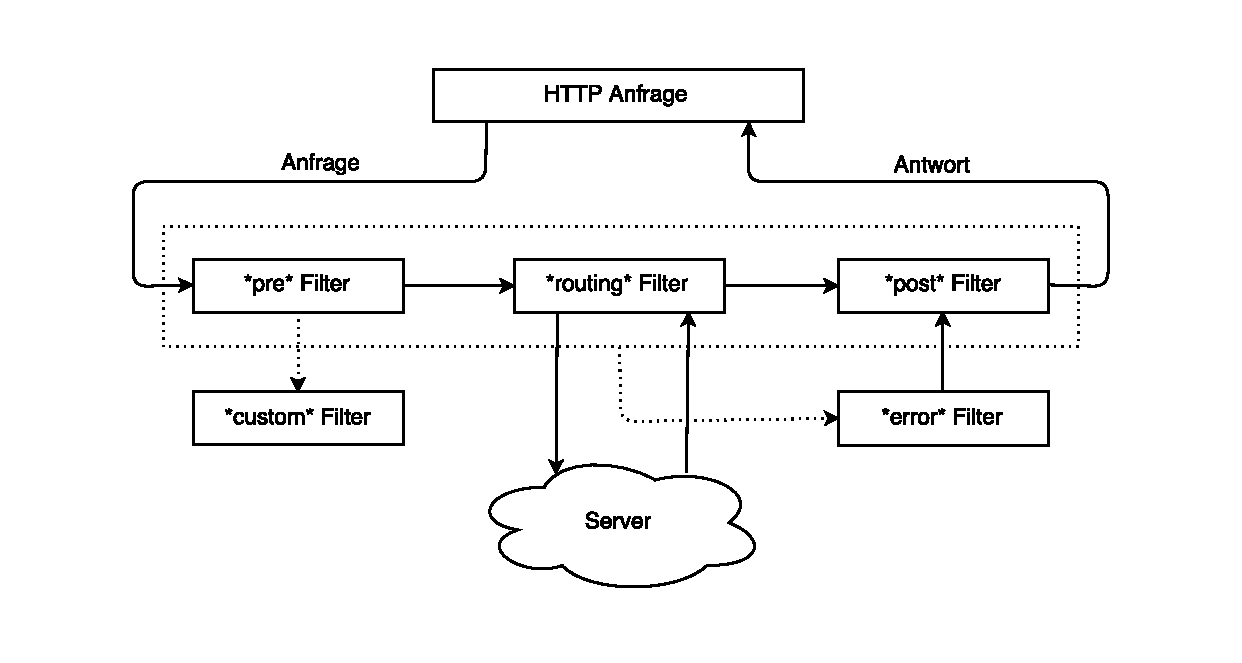
\includegraphics[width=\linewidth]{kapitel3/bilder/beispielbild}
 \caption{Beispielbild}
 \label{fig:zuul}
\end{figure}


\section{Zwei Bilder nebeneinander} 


\begin{figure}
\subfigure[Antwortzeiten]{\label{fig:antwortzeit}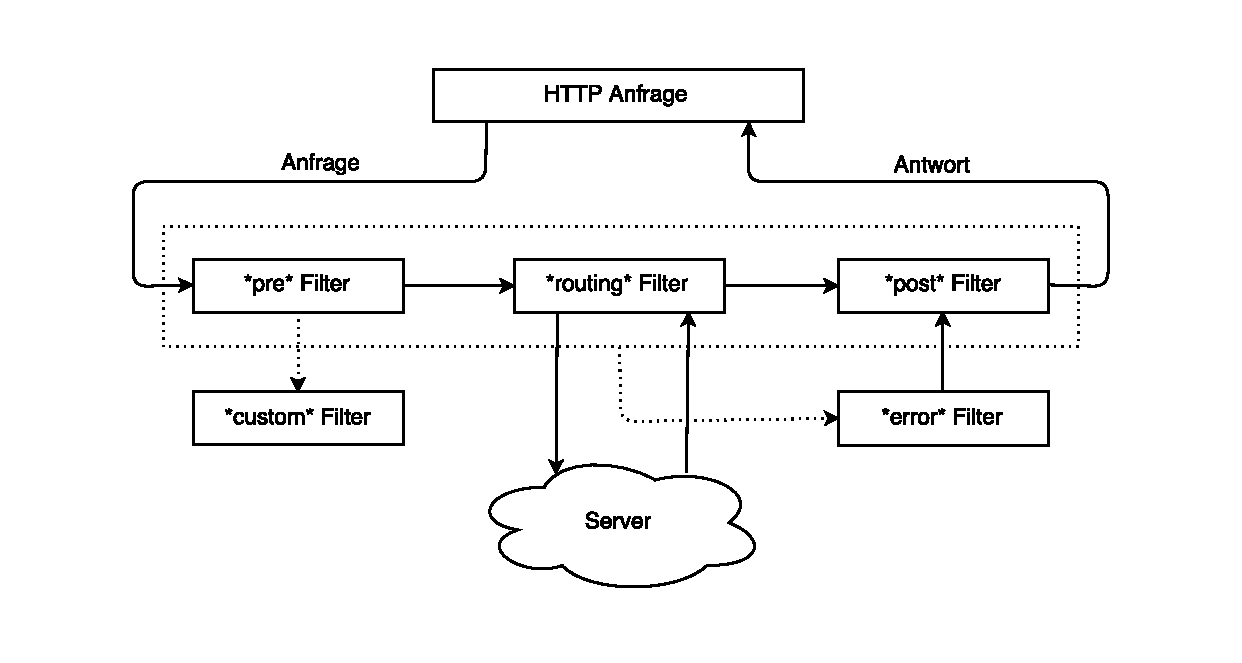
\includegraphics[width=0.50\textwidth]{kapitel3/bilder/beispielbild}}\hfill
\subfigure[prozentualer Anteil an fehlerhaften Anfragen]{\label{fig:fehler}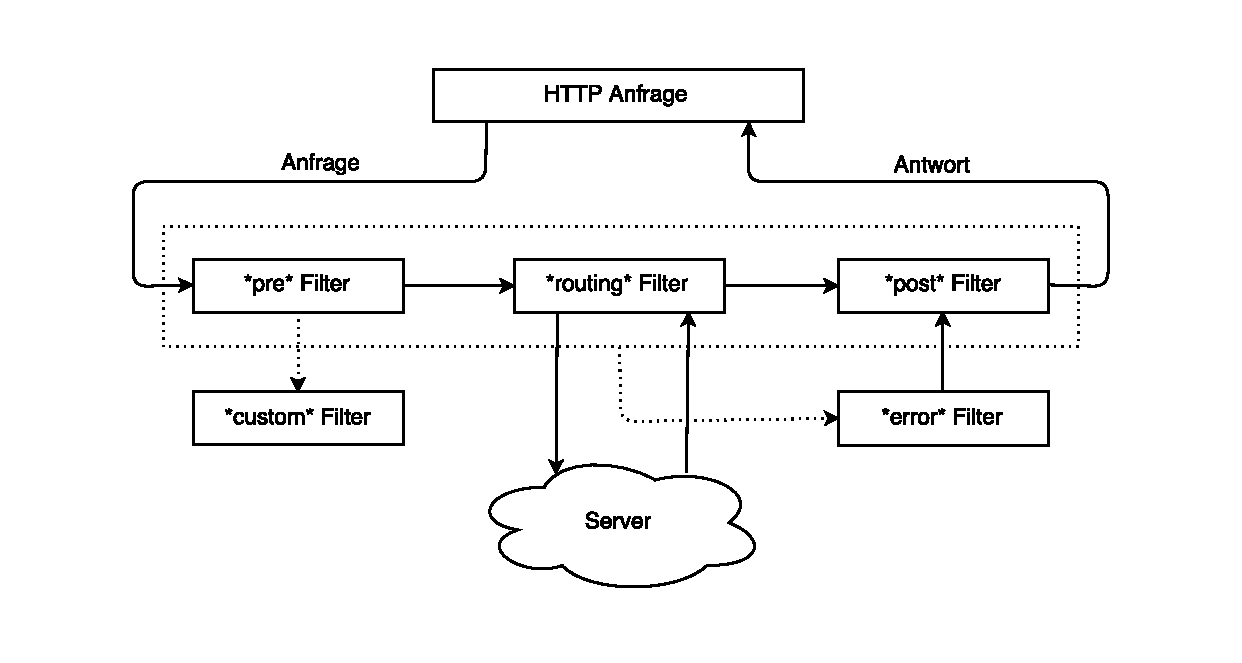
\includegraphics[width=0.50\textwidth]{kapitel3/bilder/beispielbild}}
\caption{Lasttest Szenarien}
\end{figure}

%!TEX root = ../thesis.tex

\chapter{Tabelle}

Generierbar mit \url{http://www.tablesgenerator.com/}

\section{tbd} 

\begin{table}[h]
\centering
\caption{Ergebnisse des Integartionstests in Sekunden}
\label{tab:integration}
\begin{tabular}{@{}ccccc@{}}
\toprule
Testszenario    & Start  & Registrierung & 1. Nachricht & \textbf{Gesamt} \\ \midrule
Integration\_01 & 14,598 & 10,079        & 45,449       & 70,026        \\
Integration\_02 & 14,485 & 10,108        & 54,382       & 79,088        \\
Integration\_03 & 14,498 & 10,055        & 55,125       & 79,678        \\
Integration\_04 & 14.598 & 5,361         & 36,655       & 56,614          \\ \bottomrule
\end{tabular}
\end{table}
%!TEX root = ../thesis.tex

\chapter{Quellen verwenden / verwalten}

Am besten http://www.citeulike.org/ verwenden und Expotieren als bibtex Datei.


\section{Verwenden}

Beispiel - Typ: apalike


Ergebnis: \cite{haase}

\chapter{Zukunftsprognose}\label{zukunftsprognose}

Die Standards der Web Component Technologien sind noch nicht
fertiggestellt und befinden sich momentan noch in Entwicklung. Um
allgemeingültige Standards für alle Browserhersteller zu gewährleisten,
werden sich diese vermutlich noch verändern. Jedoch werden sie dadurch
ein breites Spektrum an Zustimmung und Implementierung bekommen, da sie
eine zentrale Rolle spielen, wenn darum geht auch das Web zu einer
Plattform zu machen, für welche die Paradigmen von höheren
Programmiersprachen gelten. So soll es auch im Web möglich sein
Applikationen aus mehreren verschiedenen Komponenten, die gekapselt,
wartbar und interoperabel sind, zu entwickeln. Polymer wird dabei
weiterhin eine wichtige Rolle innehaben, da die Bibliothek das Arbeiten
mit den Web Components vereinfacht und zusätzliche Funktionalitäten
dafür leistet. Dabei könnte sogar ein Vergleich der Polymer Bibliothek
und der jQuery Bibliothek vorstellbar sein. Indem jQuery wurde zu einem
de facto Standard für das Arbeiten mit DOM Elementen, so könnte Polymer
ein Standard für das Arbeiten mit Web Components werden. Da Google
maßgeblich die Entwicklung der Standards der Web Component Technologien
vorantreibt und sich die anderen Browserhersteller teilweise daran
orientieren, könnte es sogar sein, dass zumindest Teile von Polymer zum
offiziellen Standard der Web Technologien wird. Wenn die Standards von
allen Browsern akzeptiert und implementiert wurden, sinkt auch die
Komplexität von Polymer um ein Vielfaches, da die komplette Schicht der
Polyfills wegfällt. Neben den Polyfills kann Polymer dann auf die
Nutzung des Bibliothek-internen Shady DOM verzichten und stattdessen mit
einer standardisierten, schnellen und leichtgewichtigen Version des
Shadow DOM arbeiten. Dadurch wird Polymer um einiges schneller arbeiten
und auch auf mobilen Geräten effizienten Einzug erhalten. Neben Polymer
basiert auch Angular ab Version 2.0 auf den Web Component Standards und
dessen Technologien benutzen, jedoch verfolgt Angular einen anderen
Ansatz als Polymer. Angular implementiert hierfür eigene Schicht, welche
auf die nativen Technologien zugreift und das Framework komplexer macht.
Da in Zukunft die Polyfills und der Shady DOM der Polymer Bibliothek
wegfallen, könnte Angular Polymer in sich integrieren, statt die Web
Components Standards selbst zu implementieren. Hierfür würde
beispielsweise die Micro Schicht in Frage kommen, da diese nur die
Grundfunktionalitäten für den Umgang mit den Web Components leistet.
Jedoch werden beide Bibliotheken weiterhin koexistieren und weder
Polymer Angular ersetzen oder andersrum, da Polymer nur eine
erweiterbare Bibliothek und Angular ein vollständiges Framework ist.
Beide Plattformen verfolgen daher unterschiedliche Ansätze und können
unterschiedliche Probleme lösen. Jedoch kann durch die Entwicklung der
Carbon Elemente die Polymer Bibliothek sukzessive als Framework
erweitert werden, da diese eine neue Möglichkeit bieten, wie
Applikationen strukturiert werden können. Durch sie können komplexe
Applikationen realisiert werden, da die Elemente sehr nah an der
Plattform selbst sind, was einige Vorteile mit sich bringt. So haben sie
wenige Abhängigkeiten, eine bessere Performanz, können leicht
ausgetauscht werden und bieten ein vereinfachtes Debugging an, da sie
die Tools der Plattform, statt die eines Frameworks benutzen. Polymer
kann also als eine Bibliothek mit einem optionalen Framework Plugin
verstanden werden, wobei das Framework nur die Meinung Googles'
widerspiegelt wie ein Framework funktionieren sollte. Dieses bietet, je
nach Anforderungen, Vor- und Nachteile wie jedes Andere Framework auch.
Es liegt somit weiterhin im Ermessen der Entwickler ob Angular oder
Polymer eingesetzt werden soll, oder ob sogar, bis zu einem gewissen
Grad, beides verwendet werden soll. Jedoch beschränkt sich Polymer nicht
nur auf den Einsatz in Angular, sondern kann mit jedem beliebigem
Framework kombiniert werden. Wie genau die Entwicklung von Polymer
weiter verläuft und ob sich diese auf Angular auswirken wird, liegt
jedoch ganz im Ermessen von Google.



\listoffigures
\lstlistoflistings
\listoftables

% REMOVE THIS!
\listoftodos[TODOs]
% REMOVE THIS!

\bibliographystyle{apalike}
\bibliography{library}
\end{document}

